A assinatura é utilizada em duas situações: na assinatura de uma transação; e na verificação de uma transação~\cite{overview-ahmed-2019}. Na Figura~\ref{fig:retemente-assinatura-digital} é ilustrado um exemplo em que o proprietário da conta que cede a posse realiza a assinatura da transação por meio dos passos a seguir:
\begin{enumerate}
    \item Descreve a transação com todas a informações necessárias, exceto a assinatura;
    \item Gera o valor de \textit{hash} dos dados de transação;
    \item Utiliza sua chave privada para gerar o valor de \textit{hash} da transação a partir do valor gerado no passo 2. Esse processo é chamado de encriptação;
    \item Adiciona o texto cifrado criado no item 3 à transação como sua assinatura digital.
\end{enumerate}

\begin{figure}[htb]
 \caption{Processo de assinatura digital de uma transação}
 \label{fig:retemente-assinatura-digital}
 \centering
 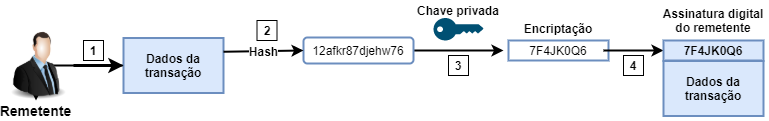
\includegraphics[scale=0.5]{figuras/remetente_assinatura_digital.png}
 \fdireta{overview-ahmed-2019}
\end{figure}

O processo de verificação de uma transação é ilustrado na Figura~\ref{fig:verifica-assinatura-digital}, no qual o nó verificador executa os seguintes passos:
\begin{enumerate}
    \item Cria o valor de \textit{hash} a partir dos dados da transação a ser verificada, com exceção da assinatura;
    \item Utiliza a chave pública da conta que está cedendo a posse para descriptografar a assinatura digital da transação. Esse processo é chamado de decriptação;
    \item Compara o valor do \textit{hash} gerado no passo 1 com o valor obtido no passo 2. Se ambos forem idênticos, então indica que a transação foi autorizada pelo proprietário da chave privada, que corresponde à chave pública que está cedendo a posse (i.e., o identificador da conta). Caso os valores não sejam idênticos, então conclui-se que o proprietário da chave privada não autorizou a transação, que é descartada. 
\end{enumerate}

\begin{figure}[htb]
 \caption{Processo de verificação da assinatura digital de uma transação}
 \label{fig:verifica-assinatura-digital}
 \centering
 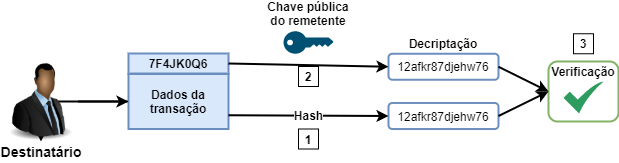
\includegraphics[scale=0.5]{figuras/verifica_assinatura_digital.png}
 \fdireta{overview-ahmed-2019}
\end{figure}